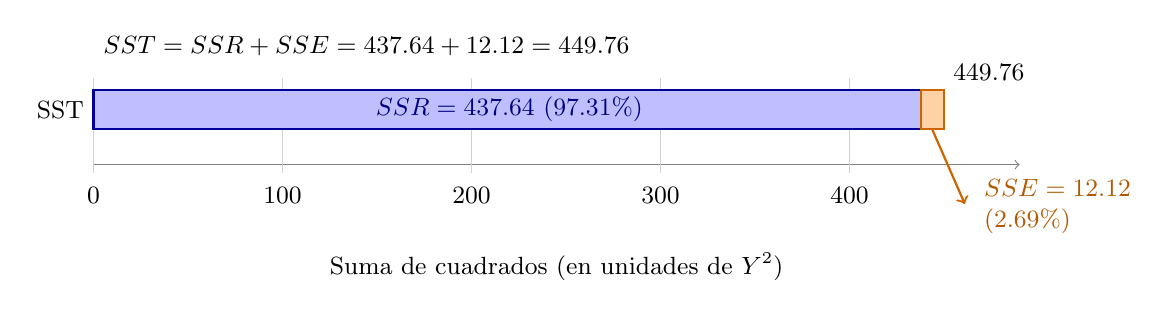
\begin{tikzpicture}[x=0.024cm,y=1cm,font=\small]
    \draw[->,gray] (0,0.55) -- (490,0.55);
    \node[anchor=west] at (0,2.05) {$SST=SSR+SSE=437.64+12.12=449.76$};
    \foreach \xx in {0,100,200,300,400} {
        \draw[gray!35] (\xx,0.45) -- (\xx,1.65);
        \node[below=2pt] at (\xx,0.45) {\xx};
    }
    \node[left,align=right] at (0,1.25) {SST};
    \draw[blue!60!black,thick,fill=blue!25] (0,1) rectangle (437.6445,1.5);
    \draw[orange!80!black,thick,fill=orange!35] (437.6445,1) rectangle (449.7600,1.5);
    \node[blue!50!black] at (220,1.25) {$SSR=437.64$ (97.31\%)};
    \draw[orange!80!black,->,thick] (443.7,1) -- (461,0.05);
    \node[orange!70!black,align=left,anchor=west] at (466,0.02) {$SSE=12.12$\\(2.69\%)};
    \node[above right] at (449.76,1.5) {$449.76$};
    \node[below] at (245,-0.45) {Suma de cuadrados (en unidades de $Y^2$)};
\end{tikzpicture}